\documentclass{standalone}
\usepackage{tikz}
\usetikzlibrary{patterns, positioning}


\begin{document}
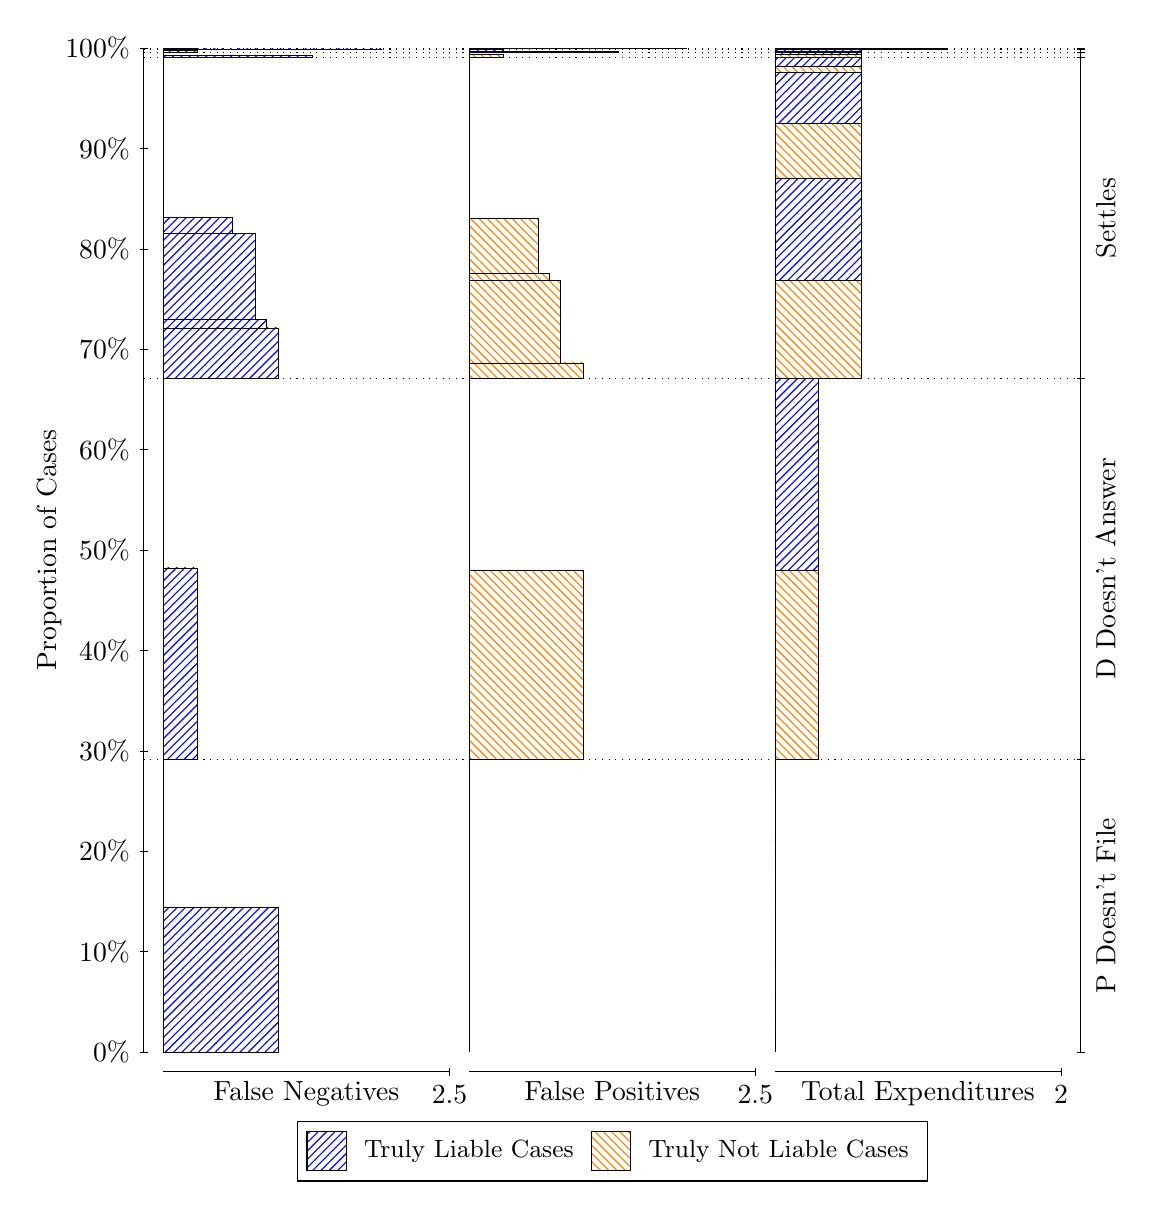
\begin{tikzpicture}
\draw[black, very thin] (1.5,1.75) -- (1.5,14.5);
\node[rotate=90, text=black, anchor=center] at (0.3, 8.125) {Proportion of Cases};
\draw[black, very thin] (1.45,1.75) -- (1.55,1.75);
\node[text=black, anchor=east] at (1.45, 1.75) {0\%};
\draw[black, very thin] (1.45,3.025) -- (1.55,3.025);
\node[text=black, anchor=east] at (1.45, 3.025) {10\%};
\draw[black, very thin] (1.45,4.3) -- (1.55,4.3);
\node[text=black, anchor=east] at (1.45, 4.3) {20\%};
\draw[black, very thin] (1.45,5.575) -- (1.55,5.575);
\node[text=black, anchor=east] at (1.45, 5.575) {30\%};
\draw[black, very thin] (1.45,6.85) -- (1.55,6.85);
\node[text=black, anchor=east] at (1.45, 6.85) {40\%};
\draw[black, very thin] (1.45,8.125) -- (1.55,8.125);
\node[text=black, anchor=east] at (1.45, 8.125) {50\%};
\draw[black, very thin] (1.45,9.4) -- (1.55,9.4);
\node[text=black, anchor=east] at (1.45, 9.4) {60\%};
\draw[black, very thin] (1.45,10.675) -- (1.55,10.675);
\node[text=black, anchor=east] at (1.45, 10.675) {70\%};
\draw[black, very thin] (1.45,11.95) -- (1.55,11.95);
\node[text=black, anchor=east] at (1.45, 11.95) {80\%};
\draw[black, very thin] (1.45,13.225) -- (1.55,13.225);
\node[text=black, anchor=east] at (1.45, 13.225) {90\%};
\draw[black, very thin] (1.45,14.5) -- (1.55,14.5);
\node[text=black, anchor=east] at (1.45, 14.5) {100\%};

\draw[black, very thin] (13.4,1.75) -- (13.4,14.5);
\draw[black, very thin] (13.35,1.75) -- (13.45,1.75);
\node[anchor=west] at (13.35, 1.75) {};
\draw[black, very thin] (13.35,5.4664) -- (13.45,5.4664);
\node[anchor=west] at (13.35, 5.4664) {};
\draw[black, very thin] (13.35,10.301) -- (13.45,10.301);
\node[anchor=west] at (13.35, 10.301) {};
\draw[black, very thin] (13.35,14.379) -- (13.45,14.379);
\node[anchor=west] at (13.35, 14.379) {};
\draw[black, very thin] (13.35,14.443) -- (13.45,14.443);
\node[anchor=west] at (13.35, 14.443) {};
\draw[black, very thin] (13.35,14.485) -- (13.45,14.485);
\node[anchor=west] at (13.35, 14.485) {};
\draw[black, very thin] (13.35,14.492) -- (13.45,14.492);
\node[anchor=west] at (13.35, 14.492) {};
\draw[black, very thin] (13.35,14.5) -- (13.45,14.5);
\node[anchor=west] at (13.35, 14.5) {};

\draw[black, very thin, pattern color=blue, pattern=north east lines] (1.75,1.75) rectangle (3.2033,3.5851);
\draw[black, very thin, pattern color=orange, pattern=north west lines] (1.75,3.5851) rectangle (1.75,5.4664);
\draw[black, very thin, pattern color=blue, pattern=north east lines] (1.75,5.4664) rectangle (2.186,7.8985);
\draw[black, very thin, pattern color=orange, pattern=north west lines] (1.75,7.8985) rectangle (1.75,10.301);
\draw[black, very thin, pattern color=blue, pattern=north east lines] (1.75,10.301) rectangle (3.2033,10.946);
\draw[black, very thin, pattern color=blue, pattern=north east lines] (1.75,10.946) rectangle (3.058,11.058);
\draw[black, very thin, pattern color=blue, pattern=north east lines] (1.75,11.058) rectangle (2.9127,12.147);
\draw[black, very thin, pattern color=blue, pattern=north east lines] (1.75,12.147) rectangle (2.622,12.346);
\draw[black, very thin, pattern color=orange, pattern=north west lines] (1.75,12.346) rectangle (1.75,14.379);
\draw[black, very thin, pattern color=blue, pattern=north east lines] (1.75,14.379) rectangle (3.6393,14.404);
\draw[black, very thin, pattern color=orange, pattern=north west lines] (1.75,14.404) rectangle (1.75,14.443);
\draw[black, very thin, pattern color=blue, pattern=north east lines] (1.75,14.443) rectangle (2.186,14.473);
\draw[black, very thin, pattern color=orange, pattern=north west lines] (1.75,14.473) rectangle (1.75,14.485);
\draw[black, very thin, pattern color=blue, pattern=north east lines] (1.75,14.485) rectangle (4.5113,14.488);
\draw[black, very thin, pattern color=orange, pattern=north west lines] (1.75,14.488) rectangle (1.75,14.492);
\draw[black, very thin, pattern color=blue, pattern=north east lines] (1.75,14.492) rectangle (2.186,14.497);
\draw[black, very thin, pattern color=orange, pattern=north west lines] (1.75,14.497) rectangle (1.75,14.5);
\draw[black, very thin, pattern color=orange, pattern=north west lines] (5.6333,1.75) rectangle (5.6333,3.6313);
\draw[black, very thin, pattern color=blue, pattern=north east lines] (5.6333,3.6313) rectangle (5.6333,5.4664);
\draw[black, very thin, pattern color=orange, pattern=north west lines] (5.6333,5.4664) rectangle (7.0867,7.8691);
\draw[black, very thin, pattern color=blue, pattern=north east lines] (5.6333,7.8691) rectangle (5.6333,10.301);
\draw[black, very thin, pattern color=orange, pattern=north west lines] (5.6333,10.301) rectangle (7.0867,10.5);
\draw[black, very thin, pattern color=orange, pattern=north west lines] (5.6333,10.5) rectangle (6.796,11.553);
\draw[black, very thin, pattern color=orange, pattern=north west lines] (5.6333,11.553) rectangle (6.6507,11.634);
\draw[black, very thin, pattern color=orange, pattern=north west lines] (5.6333,11.634) rectangle (6.5053,12.334);
\draw[black, very thin, pattern color=blue, pattern=north east lines] (5.6333,12.334) rectangle (5.6333,14.379);
\draw[black, very thin, pattern color=orange, pattern=north west lines] (5.6333,14.379) rectangle (6.0693,14.418);
\draw[black, very thin, pattern color=blue, pattern=north east lines] (5.6333,14.418) rectangle (5.6333,14.443);
\draw[black, very thin, pattern color=orange, pattern=north west lines] (5.6333,14.443) rectangle (7.5227,14.455);
\draw[black, very thin, pattern color=blue, pattern=north east lines] (5.6333,14.455) rectangle (6.0693,14.485);
\draw[black, very thin, pattern color=orange, pattern=north west lines] (5.6333,14.485) rectangle (6.0693,14.489);
\draw[black, very thin, pattern color=blue, pattern=north east lines] (5.6333,14.489) rectangle (5.6333,14.492);
\draw[black, very thin, pattern color=orange, pattern=north west lines] (5.6333,14.492) rectangle (8.3947,14.495);
\draw[black, very thin, pattern color=blue, pattern=north east lines] (5.6333,14.495) rectangle (6.9413,14.5);
\draw[black, very thin, pattern color=orange, pattern=north west lines] (9.5167,1.75) rectangle (9.5167,3.6313);
\draw[black, very thin, pattern color=blue, pattern=north east lines] (9.5167,3.6313) rectangle (9.5167,5.4664);
\draw[black, very thin, pattern color=orange, pattern=north west lines] (9.5167,5.4664) rectangle (10.062,7.8691);
\draw[black, very thin, pattern color=blue, pattern=north east lines] (9.5167,7.8691) rectangle (10.062,10.301);
\draw[black, very thin, pattern color=orange, pattern=north west lines] (9.5167,10.301) rectangle (10.607,11.553);
\draw[black, very thin, pattern color=blue, pattern=north east lines] (9.5167,11.553) rectangle (10.607,12.841);
\draw[black, very thin, pattern color=orange, pattern=north west lines] (9.5167,12.841) rectangle (10.607,13.541);
\draw[black, very thin, pattern color=blue, pattern=north east lines] (9.5167,13.541) rectangle (10.607,14.186);
\draw[black, very thin, pattern color=orange, pattern=north west lines] (9.5167,14.186) rectangle (10.607,14.268);
\draw[black, very thin, pattern color=blue, pattern=north east lines] (9.5167,14.268) rectangle (10.607,14.379);
\draw[black, very thin, pattern color=orange, pattern=north west lines] (9.5167,14.379) rectangle (10.607,14.418);
\draw[black, very thin, pattern color=blue, pattern=north east lines] (9.5167,14.418) rectangle (10.607,14.443);
\draw[black, very thin, pattern color=orange, pattern=north west lines] (9.5167,14.443) rectangle (10.607,14.455);
\draw[black, very thin, pattern color=blue, pattern=north east lines] (9.5167,14.455) rectangle (10.607,14.485);
\draw[black, very thin, pattern color=orange, pattern=north west lines] (9.5167,14.485) rectangle (11.697,14.489);
\draw[black, very thin, pattern color=blue, pattern=north east lines] (9.5167,14.489) rectangle (11.697,14.492);
\draw[black, very thin, pattern color=orange, pattern=north west lines] (9.5167,14.492) rectangle (11.697,14.495);
\draw[black, very thin, pattern color=blue, pattern=north east lines] (9.5167,14.495) rectangle (11.697,14.5);
\draw[black, dotted] (1.5,5.4664) -- (13.4,5.4664);
\draw[black, dotted] (1.5,10.301) -- (13.4,10.301);
\draw[black, dotted] (1.5,14.379) -- (13.4,14.379);
\draw[black, dotted] (1.5,14.443) -- (13.4,14.443);
\draw[black, dotted] (1.5,14.485) -- (13.4,14.485);
\draw[black, dotted] (1.5,14.492) -- (13.4,14.492);
\draw[black, very thin] (1.75,1.5) -- (5.3833,1.5);
\node[text=black, anchor=north] at (3.5667, 1.5) {False Negatives};
\draw[black, very thin] (5.3833,1.45) -- (5.3833,1.55);
\node[text=black, anchor=north] at (5.3833, 1.45) {2.5};

\draw[black, very thin] (5.6333,1.5) -- (9.2667,1.5);
\node[text=black, anchor=north] at (7.45, 1.5) {False Positives};
\draw[black, very thin] (9.2667,1.45) -- (9.2667,1.55);
\node[text=black, anchor=north] at (9.2667, 1.45) {2.5};

\draw[black, very thin] (9.5167,1.5) -- (13.15,1.5);
\node[text=black, anchor=north] at (11.333, 1.5) {Total Expenditures};
\draw[black, very thin] (13.15,1.45) -- (13.15,1.55);
\node[text=black, anchor=north] at (13.15, 1.45) {2};

\node[text=black, centered, rotate=90] at (13.72, 3.6082) {P Doesn't File};
\node[text=black, centered, rotate=90] at (13.72, 7.8838) {D Doesn't Answer};
\node[text=black, centered, rotate=90] at (13.72, 12.34) {Settles};





\draw (7.449999999999999,1.5) node[draw=none] (baseCoordinate) {};
\begin{scope}[align=center]
        \matrix[scale=0.5, draw=black, below=0.5cm of baseCoordinate, nodes={draw}, column sep=0.1cm]{
            \node[rectangle, draw, minimum width=0.5cm, minimum height=0.5cm, pattern color=blue, pattern=north east lines] {}; &
            \node[draw=none, font=\small, text=black] (B) {Truly Liable Cases}; &
            \node[rectangle, draw, minimum width=0.5cm, minimum height=0.5cm, pattern color=orange, pattern=north west lines] {}; &
            \node[draw=none, font=\small, text=black] (B) {Truly Not Liable Cases}; \\
            };
\end{scope}

\end{tikzpicture}
\end{document}